\documentclass[utf8]{beamer}
\usepackage{listings}
\usepackage[russian]{babel}
\usepackage{verbatim}
\usetheme{Malmoe}
\title{Протоколы канального уровня (Data Link Layer)}
\author {Компьютерные сети и протоколы}
\date{Лекция 6}
\begin{document}
%--------------------------------------------------------------------------------
\begin{frame}
\titlepage
\end{frame}
%--------------------------------------------------------------------------------
%--------------------------------------------------------------------------------
\section{Коммутация каналов и пакетов}
%--------------------------------------------------------------------------------
\begin{frame}
\frametitle{Коммутация каналов или пакетов}
\begin{itemize}
	\item Выделяются ли необходимые ресурсы во время установления соединения на всем пути следования данных?
	\item Возможна ли передача данных, если необходимые ресурсы не выделены?
	\item Изменяется ли маршрут следования данных за время одной сессии передачи данных?
	\item Меняется ли порядок приема блоков данных (пакетов)?
	\item Каковы требования к используемым ресурсам(задержки, вариации задержек, пропускные способности)?
	\item Используется ли промежуточное хранение данных?
\end{itemize}
\begin{center}
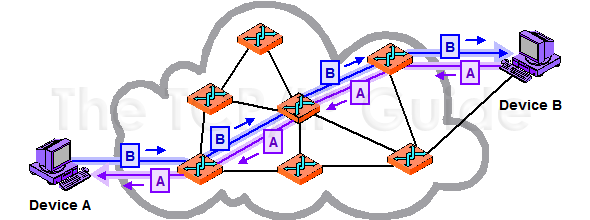
\includegraphics[width=0.6\textwidth]{pic/network.png}
\end{center}
\end{frame}
%--------------------------------------------------------------------------------
\subsection{Коммутация пакетов}
%--------------------------------------------------------------------------------
\begin{frame}
\frametitle{Особенности коммутации пакетов}
\begin{itemize}
	\item[$+$] Передача данных только по мере их поступления
	\item[?] Отдельные части одного сообщения приходят разными путями
	\begin{itemize}
		\item С одной стороны -- балансировка нагрузки в сложных топологиях (Multipath routing)
		\item Гибкое управление качеством предоставления услуг связи (Video Layered Coding)
		\item С другой -- нужно управление потоком на уровне выше сетевого
	\end{itemize}
	\item[$+$] Возможность гибкого управления доступными ресурсами
	\item[$+$] Возможность ``обхода'' неисправного узла (MANET)
	\item[$-$] Пакеты хранятся в очереди маршрутизатора
\end{itemize}
\end{frame}
%--------------------------------------------------------------------------------
\subsection{Коммутация каналов}
%--------------------------------------------------------------------------------
\begin{frame}
\frametitle{Особенности коммутации каналов}
\begin{itemize}
	\item[$+$] Выполнение жёстких требований по качеству обслуживания
	\begin{itemize}
		\item[$+$] Выделение ресурса на всем пути следования данных
		\item[$-$] Возможна большая задержка при установлении соединений
	\end{itemize}
	\item [$-$] Маршрут неизменен на протяжении всего сеанса связи
	\item [$-$] Меньшие возможности по балансировке нагрузки
	\item[$-$] Низкая устойчивость к отказам. Решение -- следить за качеством установленного канала и готовить резервный в случае деградации основного.
	\item[$+$] Отсутствует промежуточное хранение передаваемых данных.
\end{itemize}
\end{frame}
%--------------------------------------------------------------------------------
\section{Задачи канального уровня}
%--------------------------------------------------------------------------------
\begin{frame}
\frametitle{Место канального уровня в модели OSI}
\begin{center}
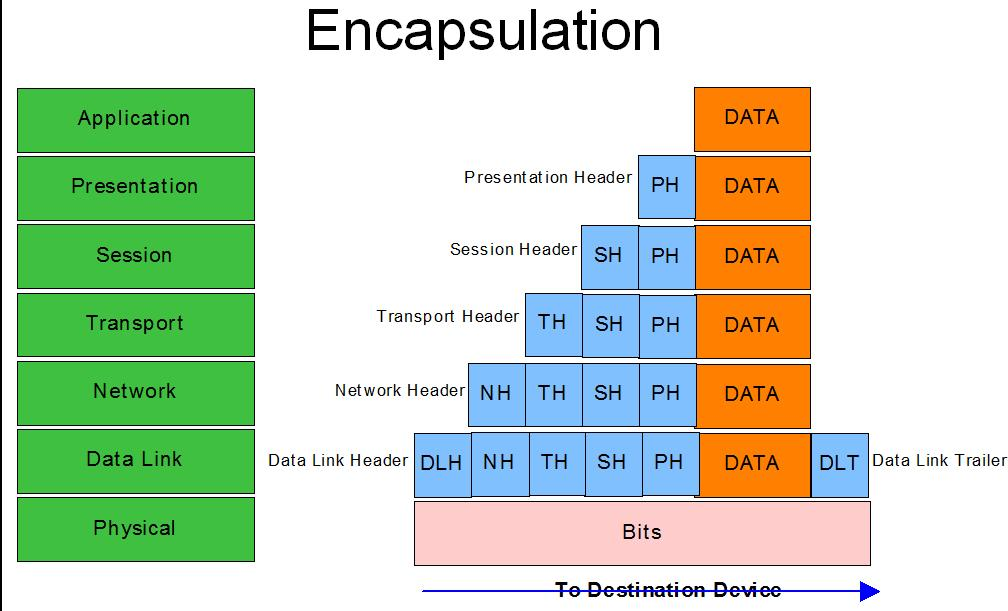
\includegraphics[width=0.6\textwidth]{pic/encapsulation.jpg}
\end{center}
Общие требования к канальному уровню:
\begin{itemize}
	\item Определение строго очерченного интерфейса для сетевого уровня
	\item Обработка ошибок передачи данных
	\item Контроль за потоком данных, исключающий затопление медленных приёмников быстрыми передатчиками
\end{itemize}
\end{frame}
%--------------------------------------------------------------------------------
\subsection{Сервисы сетевому уровню}
%--------------------------------------------------------------------------------
\begin{frame}
\frametitle{Что предоставляет нам физический уровень?}
\begin{itemize}
	\item Ошибки передачи отдельных битов. Необходима дополнительная проверка на отсутствие ошибок (CRC).
	\item Уменьшение или увеличение общего числа битов из-за ошибок передачи
	\item Сохранение последовательности передаваемых битов
	\item Задержки на распространение и конечная скорость передачи данных. Может потребовать введение дополнительных защитных интервалов.
\end{itemize}
\end{frame}
%--------------------------------------------------------------------------------
\begin{frame}
\frametitle{Требования к Data Link, определяемые физическим уровнем}
\begin{itemize}
	\item Выполнять автоматические повторные передачи (ARQ, HARQ)
	\item Выбирать оптимальную сигнально-кодовую конструкцию
	\item Динамическое назначение ресурсов с учётом состояния канала
	\item Контроль мощности и интерференции
	\item Обеспечение защиты передаваемой информации (особенно в беспроводных сетях)
\end{itemize}
\end{frame}
%--------------------------------------------------------------------------------
\begin{frame}
\frametitle{Что предоставляет канальный уровень сетевому?}
\begin{itemize}
	\item Жёсткий интерфейс для сетевого уровня (желательно для любой модульной системы)
	\item Обработка ошибок передачи потока битов
	\item Выполнение требований по качеству обслуживания
	\begin{itemize}
		\item Минимизация задержки при доставке данных, например, может конфликтовать с механизмами адаптации к условиям в канале
		\item Решение проблемы быстрого передатчика и медленного приемника
	\end{itemize}
	\item Предоставлять поток битов без ошибок
\end{itemize}
\end{frame}
%--------------------------------------------------------------------------------
\begin{frame}
\frametitle{Требования к Data Link, определяемые сетевым уровнем}
\begin{itemize}
	\item Реализовать эффективный механизм доступа к среде (MAC -- Medium Access Control)
	\item Обеспечивать приоритетную передачу данных
	\item Динамическое выделение ресурсов с учётом объёма передаваемых данных
	\item Аутентификацию абонентов и защиту информации
\end{itemize}
\end{frame}
%--------------------------------------------------------------------------------
\begin{frame}
\frametitle{LLC \& MAC}
\begin{block}{Подуровень доступа к среде (Media Access Control - MAC)}
\begin{itemize}
	\item протоколы доступа к среде;
	\item физическая адресация;
	\item очерёдность кадров и QoS;
	\item коммутация кадров и VLAN;
\end{itemize}
\end{block}
\begin{block}{Подуровень управления логической связью (Logical Link Control - LLC)}
\begin{itemize}
	\item обработка ошибок передачи данных;
	\item управление потоком данных (взаимодействие быстрых передатчиков и медленных приёмников);
	\item обеспечение служебного интерфейса для сетевого уровня
\end{itemize}
\end{block}
\end{frame}
%--------------------------------------------------------------------------------
\begin{frame}
\frametitle{Типы сервисов, предоставляемых сетевому уровню}
\begin{itemize}
	\item Без подтверждений, без установления соединения (при малой вероятности ошибки)
	\item С подтверждениями, без установления соединения (при высокой доле ошибок)
	\item С подтверждениями, ориентированный на соединение (при высокой доле ошибок)
\end{itemize}
\end{frame}
%--------------------------------------------------------------------------------
\subsection{Пример формирования кадров}
%--------------------------------------------------------------------------------
\begin{frame}
\frametitle{Способы формирования кадров}
\begin{itemize}
	\item Подсчёт количества символов
	\item Использование сигнальных стартовых и стоповых байтов с посимвольным заполнением
	\item Использование стартовых и стоповых битов с битовым заполнением
	\item Использование запрещённых сигналов физического уровня
\end{itemize}
\end{frame}
%--------------------------------------------------------------------------------
\begin{frame}
\frametitle{Подсчёт количества символов}
\begin{center}
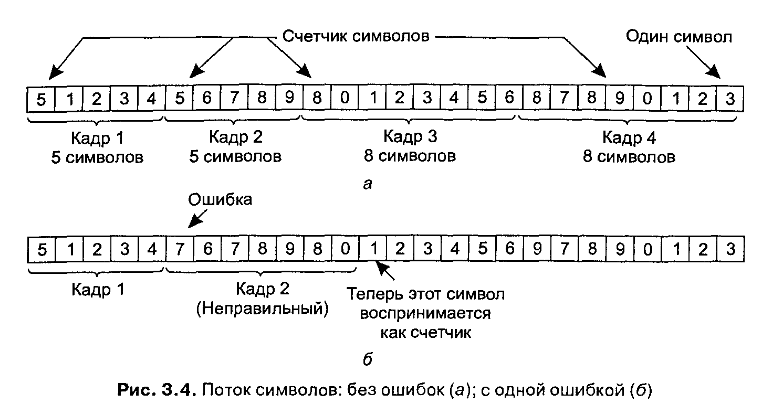
\includegraphics[width=0.9\textwidth]{pic/byte-counted-frame.png}
\end{center}
\end{frame}
%--------------------------------------------------------------------------------
\begin{frame}
\frametitle{Сигнальные символы}
\begin{center}
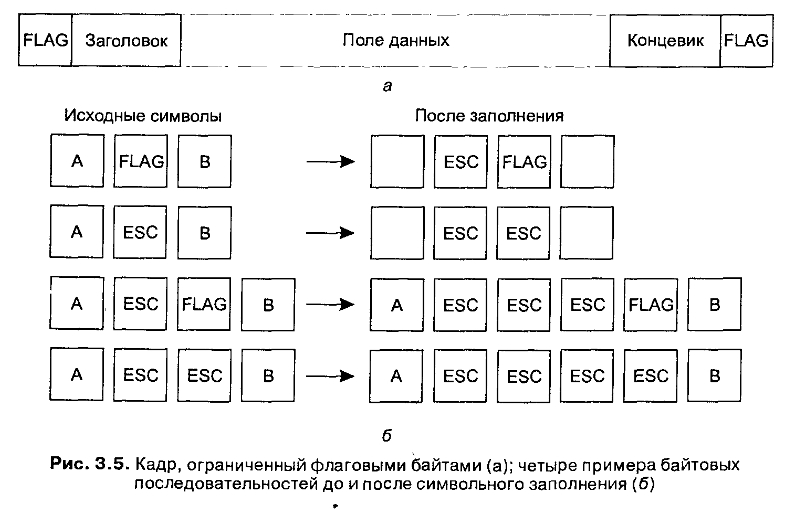
\includegraphics[width=0.9\textwidth]{pic/symbol-delimiter.png}
\end{center}
\end{frame}
%--------------------------------------------------------------------------------
\begin{frame}
\frametitle{Сигнальные биты}
\begin{center}
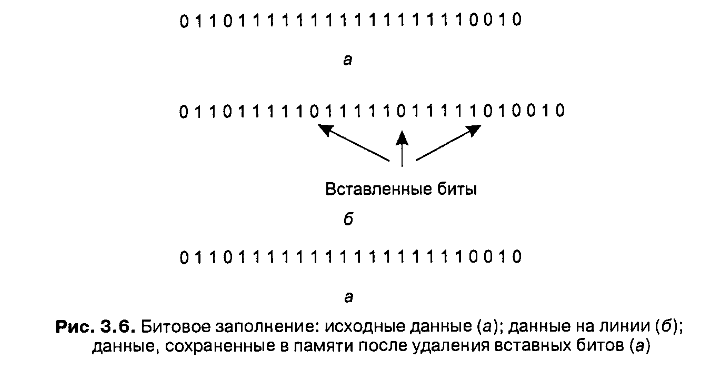
\includegraphics[width=0.9\textwidth]{pic/bi-delimiter.png}
\end{center}
\end{frame}
%--------------------------------------------------------------------------------
\subsection{Пример архитектуры канального уровня}
%--------------------------------------------------------------------------------
\begin{frame}
\frametitle{Архитектура канального уровня (IEEE 802.16)}
\begin{center}
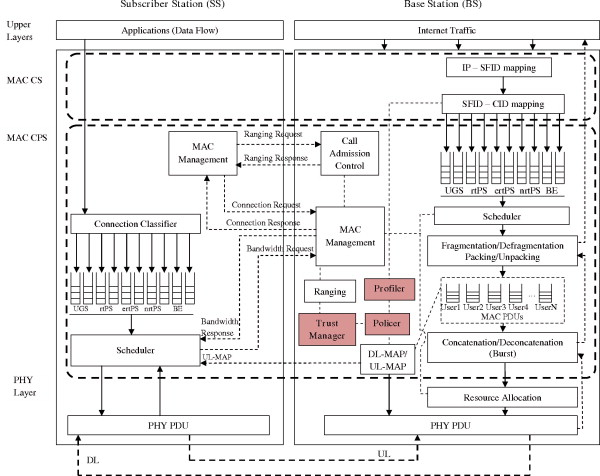
\includegraphics[width=0.8\textwidth]{pic/802-16.jpg}
\end{center}
Всегда выделяют как минимум два подуровня: передачи данных и управления доступом к среде.
\end{frame}
%--------------------------------------------------------------------------------
\section{Применение кодов}
%--------------------------------------------------------------------------------
\subsection{Исправлять или обнаруживать ошибки?}
%--------------------------------------------------------------------------------
\begin{frame}
\frametitle{Различные типы кодов для различных типов канала}
\begin{block}{Исправлять или обнаруживать ошибки?}
\begin{itemize}
 \item [Wireless] Вероятность ошибки в отдельных битах весьма высока, прямое исправление ошибок (FEC -- Forward Error correction) необходимо за счёт внесения высокой \emph{избыточности}
 \item [Wired] Вероятность ошибки низка, выгоднее повторить ``битый'' блок данных, а не вносить избыточность
\end{itemize}
\end{block}
\begin{block}{Кодовое расстояние и скорость}
Расстояние между двумя кодовыми словами:
$
|| x_1 \otimes x_2 || = d
$
Кодовое расстояние:
$
|| x_1 \otimes x_2 || \geq d, \forall x_1, x_2
$
\end{block}
\end{frame}
%--------------------------------------------------------------------------------
\subsection{Кодовое расстояние}
%--------------------------------------------------------------------------------
\begin{frame}
\frametitle{Как обеспечить кодовое расстояние?}
Кодовое расстояние обеспечивается избыточностью.
\begin{itemize}
 \item Систематический код не изменяет биты данных. Избыточность вносится только дополнительными битами
 \item В блочном коде $r$ контрольных бит вычисляются как функция $m$ битов с данными
 \item В линейных кодах рассматриваемая функция линейна
 \item Кодовое слово -- набор $n=m+r$ бит
\end{itemize}
Кодовая скорость:
$$
R=\frac{m}{n}
$$
\end{frame}
%--------------------------------------------------------------------------------
\subsection{Коды с исправлением ошибок}
%--------------------------------------------------------------------------------
\begin{frame}
 \frametitle{Коды с исправлением ошибок}
Для исправления $t$ одиночных ошибок необходимо, чтобы
$$
d \geq 2\times t + 1
$$
$A_q(n, d)$ -- максимальное возможное число кодовых слов для алфавита из $q$ символов с параметрами $n$ и $d$.
\begin{block}{Граница Хэмминга}
\end{block}
$$
A_q(n, d) \leq \frac
    {q^n}
    {\sum_{k=0}^t\left(
		    \begin{array}{c}
		    n \\
		    k \\
                    \end{array}
		 \right)
		 \cdot (q-1)^k}
\textrm{, где } t=\lfloor \frac{d-1}{2} \rfloor
$$
\end{frame}
%--------------------------------------------------------------------------------
\subsection{Коды с обнаружением ошибок}
%--------------------------------------------------------------------------------
\begin{frame}
 \frametitle{Коды с  обнаружением ошибок}
Для обнаружения $t$ одиночных ошибок необходимо, чтобы
$$
d \geq \times t + 1
$$
\begin{itemize}
 \item Код с проверкой на чётность
 \item Код с контрольными суммами
 \item Циклический избыточный код
\end{itemize}

\end{frame}
%--------------------------------------------------------------------------------
\section{Простейшие протоколы передачи данных}
%--------------------------------------------------------------------------------
\begin{frame}
\frametitle{Типы симплексных протоколов}
\begin{itemize}
  \item Неограниченный симплексный протокол
  \item Симплексный протокол с ожиданием
  \begin{itemize}
    \item[-] Обратная связь в виде подтверждений
  \end{itemize}
  \item Симплексный протокол с потерями данных и подтверждений
  \begin{itemize}
    \item[-] Порядковый номер кадра
    \item[-] Таймер для повторной отправки
  \end{itemize}
  \item Протоколы скользящего окна
\end{itemize}
\end{frame}
%--------------------------------------------------------------------------------
\subsection{Симплексный протокол для канала с шумом}
%--------------------------------------------------------------------------------
\begin{frame}
\frametitle{Симплексный протокол для канала с шумом}
\begin{itemize}
  \item Передаем ровно тогда, когда у нас появятся данные
    \begin{itemize}
    \item[-] Всегда ли принимающая сторона успеет обработать принятые пакеты?
  \end{itemize}
  \item Тогда нужна обратная связь: будем слать подтверждения.
  \begin{itemize}
    \item[-] А как же быть с потерями данных в канале?
    \item[-] Что делать с дубликатами в случае потери подтверждений?
  \end{itemize}
  \item Введем порядковый номер сообщения. Если передается каждый раз ровно один пакет, то порядковый номер состоит из одного бита.
  \item Введем тайм-аут на получение подтверждения. Если он истек, а подтверждения нет -- повторная попытка передачи.
\end{itemize}
Если задержки в канале велики, б{о}льшую часть часть времени устройство ждет ответа.
\end{frame}
%--------------------------------------------------------------------------------
\subsection{Протоколы скользящего окна}
%--------------------------------------------------------------------------------
\begin{frame}
\frametitle{Протокол скользящего окна}
\begin{center}
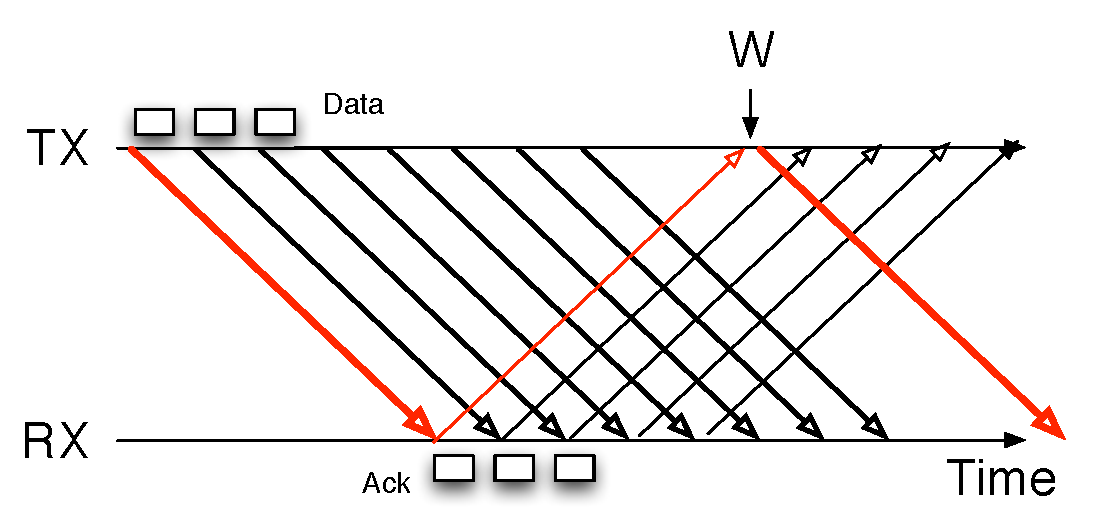
\includegraphics[width=\textwidth]{pic/window-size-example.pdf}
\end{center}
Размер окна характеризует ``ёмкость'' канала передачи!
\end{frame}
%--------------------------------------------------------------------------------
\begin{frame}
\frametitle{Протокол с однобитовым окном -- счётчики кадров}
\begin{center}
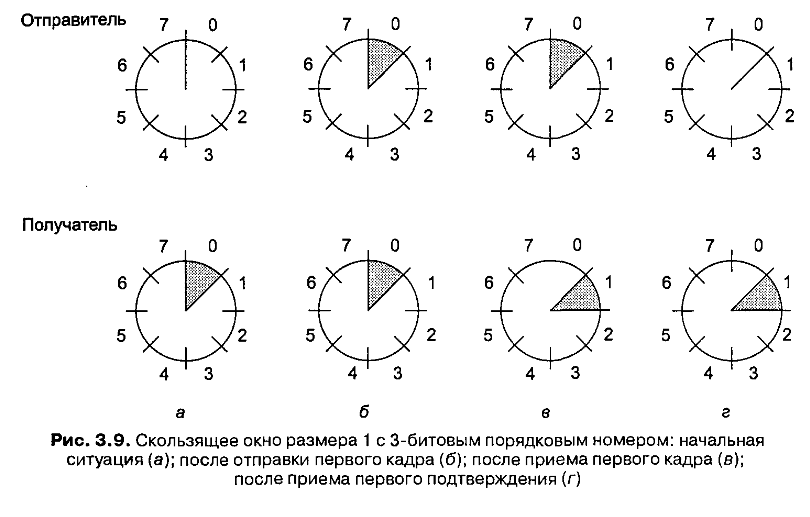
\includegraphics[width=0.9\textwidth]{pic/sliding-window.png}
\end{center}
\end{frame}
%--------------------------------------------------------------------------------
\begin{frame}
\frametitle{Протокол с однобитовым окном -- обмен данными}
\begin{center}
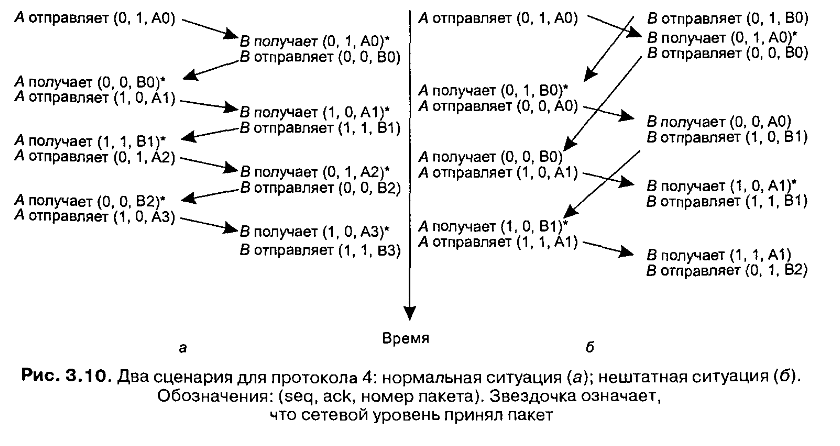
\includegraphics[width=0.9\textwidth]{pic/sliding-window-execution.png}
\end{center}
\end{frame}
%--------------------------------------------------------------------------------
\begin{frame}
\frametitle{Протокол с выборочным повтором}
\begin{center}
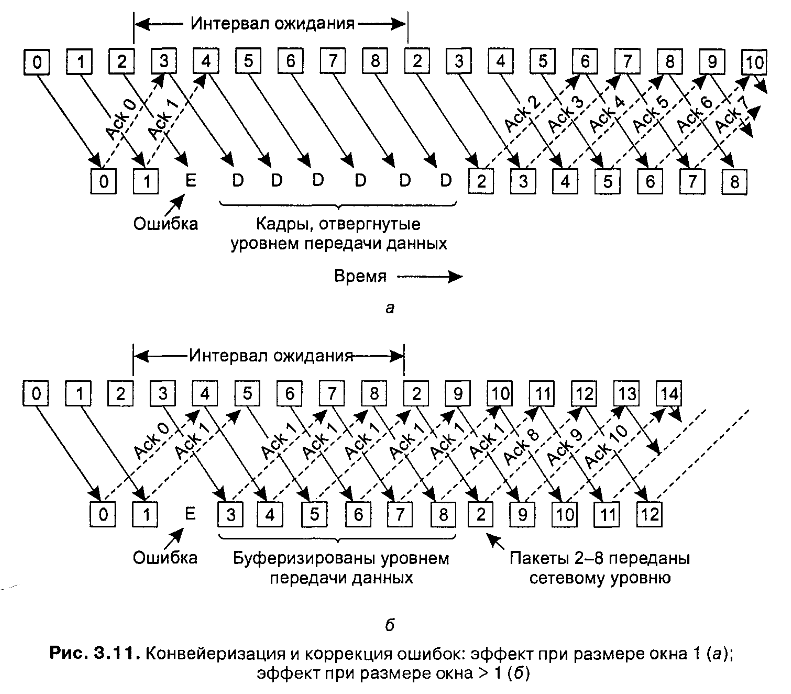
\includegraphics[width=0.8\textwidth]{pic/sliding-window-revert.png}
\end{center}
\end{frame}
%--------------------------------------------------------------------------------
\end {document}
